\documentclass{standalone}
\usepackage[T1]{fontenc}
\usepackage[utf8]{inputenc}
\usepackage{pgf,tikz}
\usepackage{pgfplots}
\pgfplotsset{compat=1.9}

\begin{document}

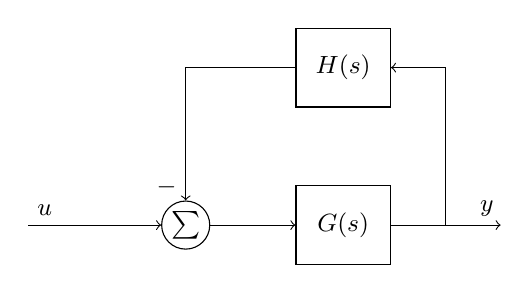
\begin{tikzpicture}[block/.style={rectangle, draw, minimum width=12mm, minimum height=10mm},
  sumnode/.style={circle, draw, inner sep=1pt},
  node distance=20mm]
  \small 
  \node[coordinate] (input) {};
  \node[sumnode, right of=input] (sum) {$\sum$};
  \node[block, right of=sum] (G) {$G(s)$};
  \node[block, above of=G,]  (H) {$H(s)$};
  \node[coordinate, right of=G] (output) {};
 
  \draw[->] (input) -- node[ very near start, above] {$u$} (sum);
  \draw[->] (sum) -- node[ very near start, left] {} (G);
  \draw[->] (G) -- node[coordinate, pos=0.5,] (meas) {} node[ very near end, above] {$y$} (output);
  \draw[->] (meas) |- (H);
  \draw[->] (H) -| node[pos=0.95, left] {$-$} (sum);


\end{tikzpicture}
\end{document}
